%%%%%%%%%%%%%%%%%%%%%%%%%%%%%%%%%%%%%%%%%
% University/School Laboratory Report
% LaTeX Template
% Version 3.1 (25/3/14)
%
% This template has been downloaded from:
% http://www.LaTeXTemplates.com
%
% Original author:
% Linux and Unix Users Group at Virginia Tech Wiki 
% (https://vtluug.org/wiki/Example_LaTeX_chem_lab_report)
%
% License:
% CC BY-NC-SA 3.0 (http://creativecommons.org/licenses/by-nc-sa/3.0/)
%
%%%%%%%%%%%%%%%%%%%%%%%%%%%%%%%%%%%%%%%%%

%----------------------------------------------------------------------------------------
%	PACKAGES AND DOCUMENT CONFIGURATIONS
%----------------------------------------------------------------------------------------

\documentclass{article}

\usepackage[version=3]{mhchem} % Package for chemical equation typesetting
\usepackage{siunitx} % Provides the \SI{}{} and \si{} command for typesetting SI units
\usepackage{graphicx} % Required for the inclusion of images
\usepackage{natbib} % Required to change bibliography style to APA
\usepackage{amsmath} % Required for some math elements 
\usepackage{epsfig}
\usepackage{subfigure}
\usepackage{epstopdf}
\usepackage{multirow}
\usepackage{ctex}
\epstopdfsetup{outdir=./Figures/}
\graphicspath{{./Figures/}}
\setlength\parindent{0pt} % Removes all indentation from paragraphs

\renewcommand{\labelenumi}{\alph{enumi}.} % Make numbering in the enumerate environment by letter rather than number (e.g. section 6)

%\usepackage{times} % Uncomment to use the Times New Roman font

%----------------------------------------------------------------------------------------
%	DOCUMENT INFORMATION
%----------------------------------------------------------------------------------------

\title{计算机组成原理16位流水CPU实验报告
} % Title

\author{
小组编号 402\\
计24 田博 2012011346\\
计24 裘捷中 2012011345\\
计24 柯均洁 2012011335
} % Author name

\date{\today} % Date for the report

\begin{document}

\maketitle % Insert the title, author and date

\setcounter{tocdepth}{3} % Set the depth of the table of contents to show sections and subsections only

\tableofcontents % Print the table of contents

%\begin{center}
%\begin{tabular}{l r}
%Date Performed: & January 1, 2012 \\ % Date the experiment was performed
%Partners: & James Smith \\ % Partner names
%& Mary Smith \\
%Instructor: & Professor Smith % Instructor/supervisor
%\end{tabular}
%\end{center}

% If you wish to include an abstract, uncomment the lines below
% \begin{abstract}
% Abstract text
% \end{abstract}

\section{实验目的}
\begin{itemize}
\item 加深对计算机系统知识的理解
\item 进一步理解和掌握流水线结构计算机各部件组成及内部工作原理
\item 掌握计算机外部输入输出的设计
\item 培养硬件设计和调试的能力
\end{itemize}

\section{实验环境}
\begin{itemize}
\item 硬件环境:
	\begin{itemize}
	\item 安装有Windows7或以上操作系统的微机
	\item THINPAD教学计算机
	\end{itemize}
\item 软件环境:
	\begin{itemize}
	\item FPGA开发工具软件XILINX ISE 12.3或以上
	\item THINPAD教学计算机软件包,包括监控程序、终端程序、数据通信程序、汇编程序等
	\end{itemize}
\end{itemize}

\section{实验内容}
\begin{itemize}
\item 指令系统设计
	\begin{itemize}
	\item 设计并实现5级指令流水的CPU,实现基本指令集和扩展指令集
	\item 能够运行教学计算机监控程序
	\item 能够运行包含5条扩展指令的用户程序
	\end{itemize}
\item 控制器设计
	\begin{itemize}
	\item 实现延时槽
	\item 适当应用数据旁路、冲突检测等方式解决流水线“冲突”问题,提高流水线的效率
	\end{itemize}
\item 内存管理设计
	\begin{itemize}
	\item 内存地址分配应满足监控程序使用内存的要求
	\end{itemize}
\item 输入输出设计
	\begin{itemize}
	\item 完成对串口的访问
	\end{itemize}
\item 监控程序装入
	\begin{itemize}
	\item 使用数据通信程序FlashAndRam,将Kernel的二进制代码直接装入到内存RAM
	\end{itemize}
\item 扩展功能实现:VGA 
\end{itemize}


\section{实验设计与实现}

\subsection{数据通路和控制信号设计图图}

\begin{figure}[h]
%\centering
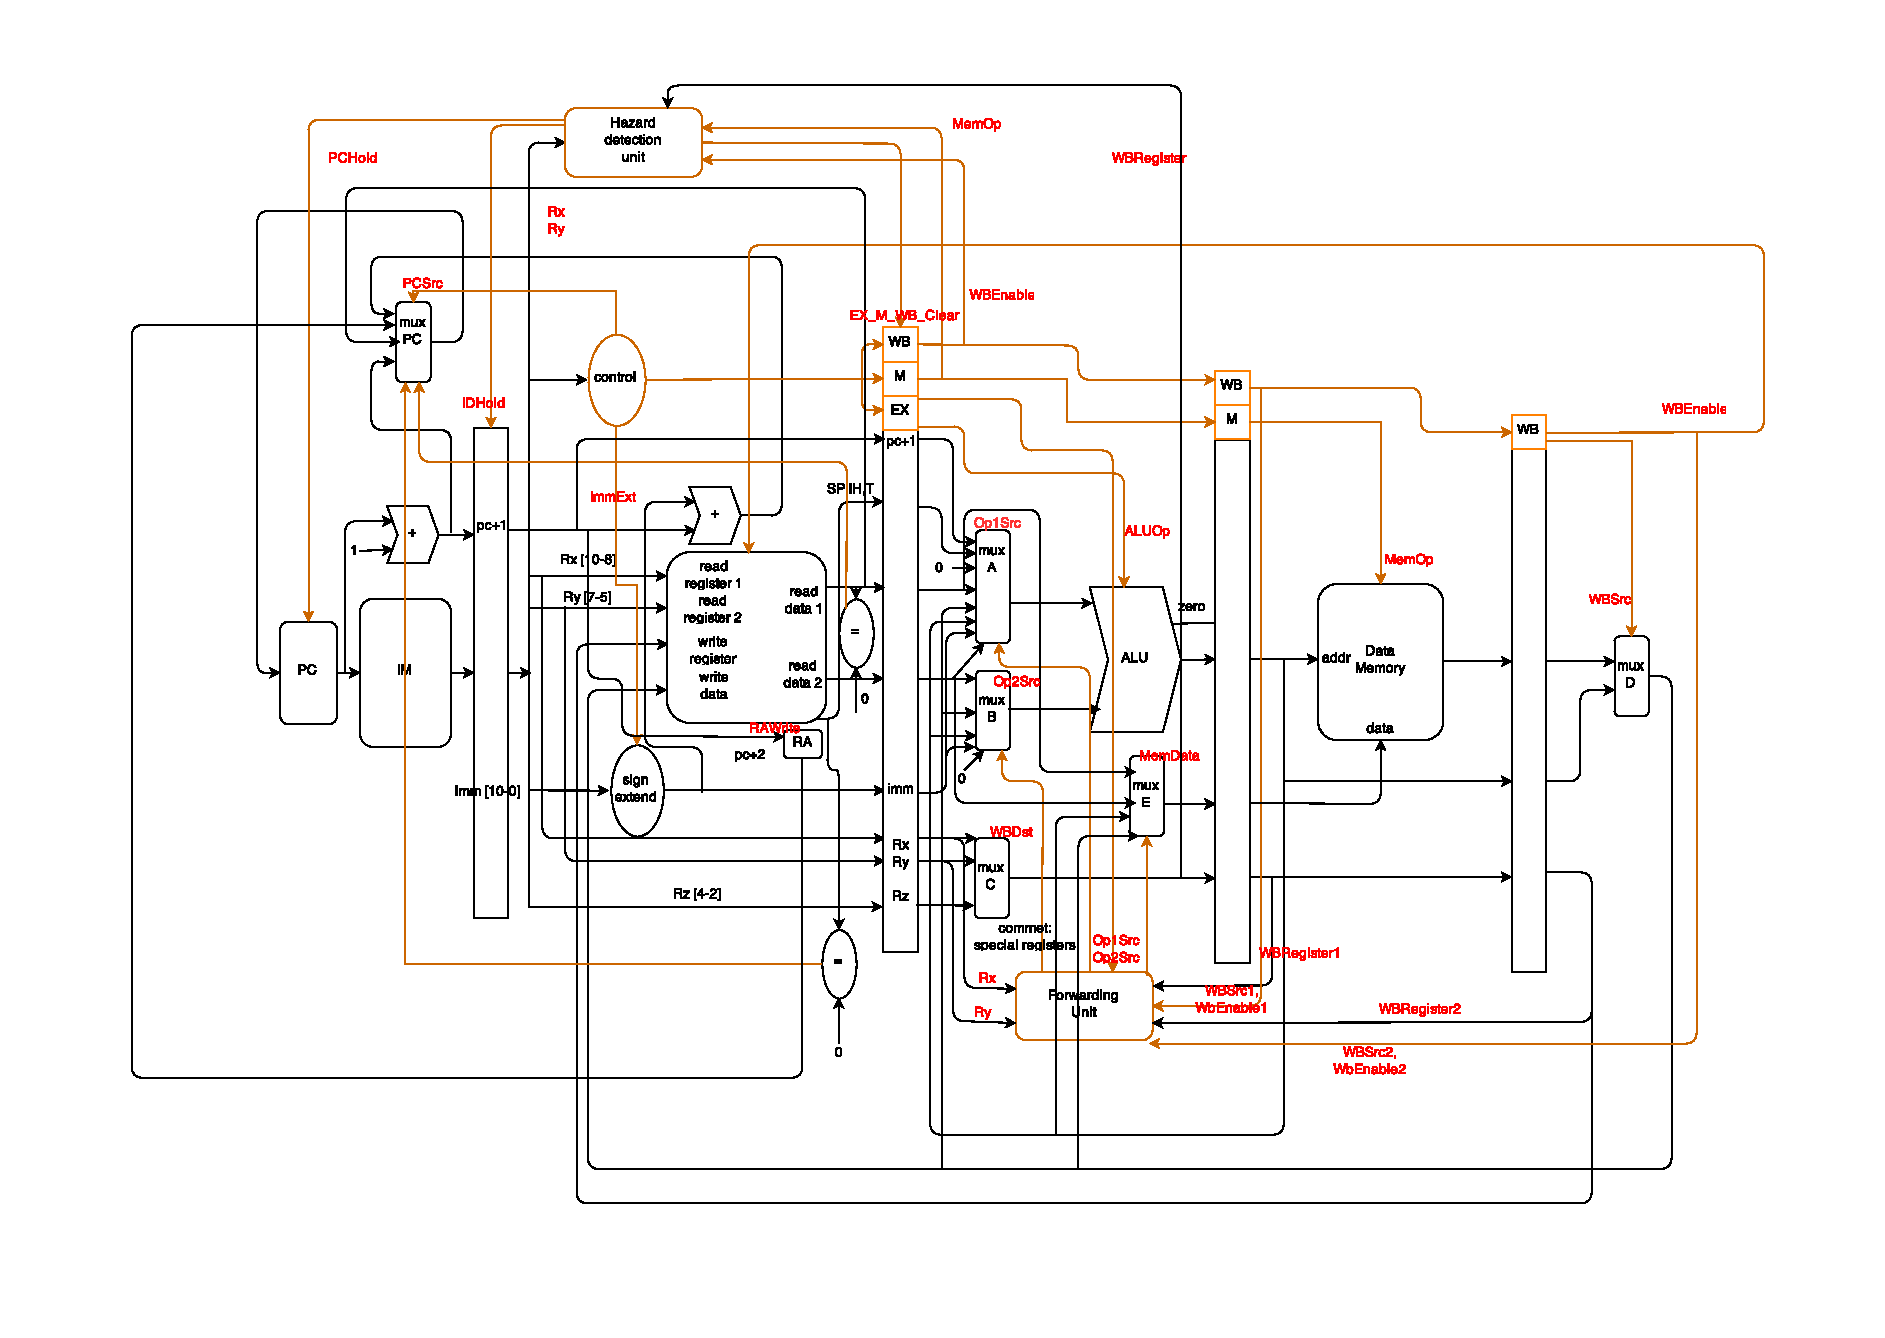
\includegraphics[width=1.1\columnwidth]{datapath.pdf}
\caption{数据通路和控制信号设计图}
\label{fig:datapath}
\end{figure}

\subsection{IF阶段}

\subsubsection{MUX\_PC}
\label{subsubsec:pc}
\paragraph{单元描述}
\paragraph{输入信号}
\begin{itemize}
\item PCSrc:控制MUX\_PC来选择下一个PC的取值,是顺序执行的PC+1或者是新的PC地址。取值情况为:
	\begin{itemize}
	\item PC1:等于PC+1,即顺序执行
	\item B:跳转到新地址Branch
	\item RA:跳转地址来自RA寄存器
	\item Rx:跳转地址来自Rx寄存器
	\item Rx\_0:R[x]=0时跳转到新地址Branch
	\item Rx\_1:R[x]!=0时跳转新地址Branch
	\item T\_0:T寄存器=0时跳转新地址Branch
	\end{itemize}
\item PCHold:
	\begin{itemize}
	\item PC是否保持,由Hazard Detect Unit控制。若PCHold为1,则保持原有的PC不变;若PCHold为0,则选择计算结果作为新的PC
	\end{itemize}
\end{itemize}
\paragraph{输出信号}
\begin{itemize}
\item Ret: 根据输入和控制信号输出相应的PC值
\end{itemize}

\subsubsection{RamHandler指令单元}

由于在我们的实现中,指令内存和数据内存使用的时同一块RAM(RAM2),所以对于RAM的操作我们统一用RamHandler这个entity来封装实现。
为保证说明时的一致性,我们会在\ref{subsec:mem}详细对这一模块进行描述。

\subsection{ID阶段}

\subsubsection{Controller控制单元}

\paragraph{单元描述}
\begin{itemize}
	\item 进行指令译码,产生之后阶段所需要的控制信号
	\item 默认初始化为NOP指令,即不写寄存器、不读内存 
\end{itemize}

\paragraph{输入信号}
\begin{itemize}
	\item INS: 16位指令 
\end{itemize}

\paragraph{输出信号}
\subparagraph{IFRegs}
IF阶段的控制信号,控制指令的跳转,由以下具体信号组成:
\begin{itemize}
	\item PCSrc : 选择哪个地址作为下一个PC,取值详见\ref{subsubsec:pc}
\end{itemize}
\subparagraph{IDRegs}
ID阶段的控制信号,由以下具体信号组成:
\begin{itemize}
	\item ImmExt:立即数扩展的形式
	\item RAWrite:是否要写RA寄存器
\end{itemize}
\subparagraph{EXRegs}
EX阶段的控制信号,由以下具体信号组成:
\begin{itemize}
	\item Op1Src: ALU操作数1的来源,MUX\_A选择信号
	\item Op2Src: ALU操作数2的来源,MUX\_B选择信号
	\item WBDst: 写回的目标寄存器。
	\item ALUOp:ALU的操作码。 
	\item MemData:读内存的地址来源寄存器
\end{itemize}
\subparagraph{MRegs}
MEM阶段的控制信号,由以下具体信号组成:
\begin{itemize}
	\item MemOp:内存的读取,取值为: 
		\begin{itemize}
			\item None:非访存操作
			\item Read:读取内存数据
			\item Write:写内存数据
		\end{itemize}
\end{itemize}

\subparagraph{WBRegs}
WB阶段的控制信号,由以下具体信号组成:
\begin{itemize}
	\item WBSrc:写回寄存器数据来源于ALU输出还是内存读取输出
	\item WBEnable:是否写回
\end{itemize}


\subsubsection{RegisterGroup寄存器组}

\paragraph{单元描述}

\subparagraph{维护寄存器组}
将编程可见的8个通用寄存器(编号0-7)以及T寄存器(编号8)、IH寄存器(编号9)、SP寄存器(编号10)封装到一起。RA寄存器单独存放。
\subparagraph{寄存器值的写入}
在一个CPU周期的上升沿写,写入的寄存器编号为write\_reg,由写回阶段的写回目的地信号WB\_Register\_out\_data.WBDst指定。
\subparagraph{寄存器值的读取}
读取的寄存器号由read\_reg1和read\_reg2指定。特殊寄存器由专门的输出信号regIH\_out、regSP\_out、regT\_out读出

\paragraph{输入信号}
\begin{itemize}
	\item clk:CPU时钟
	\item write\_enable:控制寄存器堆是否写入 
	\item read\_reg1、read\_reg2:要读取的两个寄存器编号
	\item write\_reg:要写入的寄存器编号 
	\item write\_data:要写入的值
\end{itemize}

\paragraph{输出信号}
\begin{itemize}
	\item reg1\_data、reg2\_data:读取的寄存器数据
	\item reg\_0\_out到reg7\_out、regIH\_out、regSP\_out、regT\_out:8个通用寄存器及Rsp、Rih寄存器的数据 
\end{itemize}

\subsubsection{RA寄存器}

\paragraph{单元描述}
由于RA寄存器用于特殊的JALR和JRRA指令,因此单独维护RA寄存器的读写。

\paragraph{输入信号}
\begin{itemize}
	\item clk:CPU时钟周期
	\item RAWrite:是否写RA寄存器 
	\item write\_data:用于写RA寄存器的数据,PC+1
\end{itemize}
\paragraph{输出信号}
\begin{itemize}
	\item RA:当前RA寄存器的值
\end{itemize}
\paragraph{实现细节}
由于写RA时只需要写入RPC,所以将输入的写数据write\_data取为PC+1,若需要写RA则将write\_data加1得到RPC写入RA寄存器

\subsubsection{SignExtend / ZeroExtend 符号/零扩展单元}

\paragraph{单元描述}

计算不同指令符号扩展或零扩展之后的16位立即数

\paragraph{输入信号}
\begin{itemize}
	\item imm\_in: 输入的需要扩展的立即数(11位)
	\item ImmExt: 由于不同指令存放立即数的长度和扩展类型是不同的,因此需要该控制信号标明立即数的位数及需要扩展的类型取值类型为
	\begin{itemize}
	\item ImmExt\_Sign\_7 立即数为7-0位,符号扩展
	\item ImmExt\_Sign\_3立即数为3-0位,符号扩展
	\item ImmExt\_Sign\_10立即数为10-0位,符号扩展
	\item ImmExt\_Sign\_4立即数为4-0位,符号扩展
	\item ImmExt\_Shift\_4\_2立即数为4-2位(相当于右移)
	\item ImmExt\_Zero\_7立即数为7-0位,零扩展
	\end{itemize}
\end{itemize}

\paragraph{输出信号}
\begin{itemize}
	\item imm\_out:16位扩展立即数
\end{itemize}

\subsubsection{Forwarding Unit 转发单元}

\paragraph{单元描述}

利用数据旁路技术来解决部分数据冒险

\paragraph{输入信号}
\begin{itemize}
	\item Rx, Ry
	\item Op1Src:ALU操作数来源,MUX\_A选择信号
	\item Op2Src:ALU操作数来源,MUX\_B选择信号
	\item wbsrc:当前指令要写回的结果来源于ALU的输出或访存结果 
	\item wbregister1:EX\_MEM阶段的那条指令写回的寄存器
	\item wbregister2:MEM\_WB阶段的那条指令写回的寄存器 
	\item wbenable1:EX\_MEM阶段的那条指令是否写寄存器	
	\item wbenable2:MEM\_WB阶段的那条指令是否写寄存器 
	\item memdata:写内存的数据来源
\end{itemize}
\paragraph{输出信号}
\begin{itemize}
	\item forwarda、forwardb、forwarde:MUX\_A、MUX\_B、MUX\_E是否使用forward数据及forward数据的来源,类型均为ForwardType,取值为:
	\begin{itemize}
		\item Forward\_None:不需要使用转发数据
		\item Forward\_From\_M\_WB:转发数据来自MEM\_WB阶段寄存器,也就是上一条指令的ALU计算结果
		\item Forward\_From\_WB:转发数据来自上一个MEM阶段得到的准备写回的数据,即访存所得数据
	\end{itemize}
\end{itemize}



\paragraph{实现细节}
\begin{itemize}
	\item 转发数据的来源有两个,一个是上一个阶段ALU的计算结果,另外一个是访存的结果。选择类型通过ForwardType的类型来指定
	\item 转发ALU计算结果的条件:
	\begin{itemize}
		\item 写回寄存器编号wbregister1与rx/ry/SP\_index/IH\_index相同
		
		\item 对应的写回使能wbenable1置1
		
		\item 当前指令写回的数据来源于ALU的计算结果
	\end{itemize}
	\item 转发访存结果的条件:
	\begin{itemize}
		\item 转发ALU计算结果的调节不满足
		\item 写回寄存器编号wbregister2与rx/ry/SP\_index/IH\_index相同
		\item 对应的写回使能wbenable2置1
	\end{itemize}
	\item 有些指令写回寄存器的值不是两个数操作后的运算结果,而是零扩展、某些寄存器值等等,可以将这种情况看做一个数和0相加,这样写回寄存器的值也可以看做ALURes来统一处理
\end{itemize}

\subsubsection{Hazard Detector 冒险测试单元}

\paragraph{单元描述}
\begin{itemize}
	\item 解决访存指令LW引起的数据冒险,若下一条指令Ex阶段需要使用LW指令的访存数据,则需要暂停流水,也就是插入NOP。
	
	\item 此外,由于指令和数据均存放在RAM2中,所以访问数据时也需要暂停流水 
\end{itemize}

\paragraph{输入信号}
\begin{itemize}
	\item wbenable:是否写回
	
	\item memop:ex阶段指令访存的操作,取/读/不操作 

	\item memop2:mem阶段指令访存的操作,取/读/不操作
	
	\item idrx、idry:id阶段的rx和ry 

	\item wbregister:写回的寄存器
	
	\item MemAddr:访问的内存地址 
\end{itemize}

\paragraph{输出信号}
\begin{itemize}
	\item exmwbclear:是否清空EX,MEM,WB阶段的信号
	
	\item Idhold:是否保持ID阶段指令 

	\item Pchold:是否保持PC
\end{itemize}

\paragraph{实现细节}

\subparagraph{LW引起的数据冒险暂停流水线作用条件}
	\begin{itemize}
	\item 需要写回寄存器,即wbenable置1
	\item memop==MemOp\_read,即这是一条LW指令
	\item idrx或idry与写回寄存器wbregister相等
	\end{itemize}

\subparagraph{MEM阶段访问RAM2暂停流水线作用条件}
由于我们把IM和DM都放在了RAM2上,所以一旦涉及到RAM2的读写操作,就无法正常读出下一条指令,因此必须暂定流水线一个周期。具体调节为:
	\begin{itemize}
		\item MEM阶段有读写RAM2操作
		\item 访存地址不是串口相关地址
	\end{itemize}


\subsection{EX阶段}

\subsubsection{ALU模块}

\paragraph{单元描述}

提供运算结果

\paragraph{输入信号}
\begin{itemize}
	\item Op1:ALU操作数1
	\item Op2:ALU操作数2 
	\item ALUOp:ALU的运算类型控制信号,取值为:
		\begin{itemize}
		\item ALUOp\_Plus:Op1 + Op2
		\item ALUOp\_And:Op1 and Op2
		\item ALUOp\_Sub:Op1 - Op2
		\item ALUOp\_Or:Op1 or Op2
		\item ALUOp\_SLL:Op1 逻辑左移Op2
		\item ALUOp\_SRA:Op1算术右移Op2
		\item ALUOp\_If\_Less:若Op1 < Op2则置为1,否则置为0
		\end{itemize}
\end{itemize}


\paragraph{输出信号}
\begin{itemize}
	\item ALURes:运算结果
\end{itemize}
	
\subsubsection{MUX\_A/MUX\_B:ALU操作选择器}
	
\paragraph{MUX\_A}
	
\subparagraph{单元描述}
选择数据作为ALU的第一个操作数

\subparagraph{输入信号}
	
\begin{itemize}
	\item 由EX阶段锁存器给出的的Op1src,指定操作数来源取值为
		\begin{itemize}
			\item Rx:R[x]
			\item Ry:R[y]
			\item SP:SP寄存器
			\item IH:IH寄存器
			\item Imm:16位立即数
			\item PC1:PC+1
		\end{itemize}
	\item 由Forward Unit产生的ForwardA,指定是否使用转发数据及转发数据来源。
	\item Rx, Ry SP, IH:分别表示相应寄存器的值
	\item Imm:立即数
	\item PC1:PC+1的值
	\item Data\_From\_WB:从WB阶段写回的数据
	\item Data\_From\_M\_WB:从MEM阶段写回的数据
\end{itemize}

\subparagraph{输出信号}
根据ForwardA的值以及控制信号Op1src选择对应的输入值作为该多路选择器的输出。
	
\paragraph{MUX\_B}
	
\subparagraph{单元描述}
选择数据作为ALU的第二个操作数
	
\subparagraph{输入信号}
\begin{itemize}
\item 由EX阶段锁存器给出的的Op2src,指定操作数来源,取值为
\begin{itemize}
\item Ry:R[y]
\item Imm:16位立即数
\item 0:零
\end{itemize}
\item Ry:R[y]
\item Imm:立即数
\item Data\_From\_WB:从WB阶段写回的数据
\item Data\_From\_M\_WB:从MEM阶段写回的数据
\item 由Forward Unit产生的ForwardB,指定是否使用转发数据及转发数据来源。
\end{itemize}
\subparagraph{输出信号}
根据ForwardB的值以及控制信号Op2src选择对应的输入值作为该多路选择器的输出。

\subsubsection{MUX\_C:写回寄存器编号选择器}	
\paragraph{单元描述}
选择写回寄存器的来源,由WBDst控制
\paragraph{输入信号}
\begin{itemize}
\item Rx, Ry, Rz
\item EX阶段锁存器给出的WBDst信号,取值为:
\begin{itemize}
\item Rx:写回rx字段的寄存器
\item Ry:写回ry字段的寄存器
\item Rz:写回rz字段的寄存器
\item SP:写回SP寄存器
\item IH:写回IH寄存器
\item T:写回T寄存器
\end{itemize}
\end{itemize}

\subparagraph{输出信号}
根据局WBDst选择对应的输入值作为该多路选择器的输出。

\subsubsection{MUX\_E:访存地址来源选择器}
\paragraph{单元描述}
选择访存地址的来源寄存器
\paragraph{输入信号}
\begin{itemize}
\item Rx, Ry
\item Data\_From\_WB:从WB阶段写回的数据
\item Data\_From\_M\_WB:从MEM阶段写回的数据
\item 由EX阶段锁存器给出的MemData信号,取值为:
\begin{itemize}
	\item Rx:来源于rx字段的寄存器
	\item Ry:来源于ry字段的寄存器
\end{itemize}
\item Forward Unit产生的ForwardE,指定是否使用转发数据及转发数据来源
\end{itemize}
\subparagraph{输出信号}
根据ForwardE的值以及控制信号MemData选择对应的输入值作为该多路选择器的输出。
	
		
\subsection{MEM阶段}
\label{subsec:mem}		
\subsubsection{RamHandler指令数据存储器}
		
\paragraph{单元描述}
控制Ram中指令的读入和数据的读写,以及串口的访问
		
\paragraph{输入信号}
		\begin{itemize}
			\item clk 时钟
			\item Memop 
			\item dm\_addr
			\item im\_addr 
			\item data\_in
			\item com\_data\_ready 
			\item com\_tbre
			\item com\_tsre 
			\item ram1\_data\_out
			\item ram2\_data\_out 
		\end{itemize}
		
\paragraph{输出信号}
		\begin{itemize}
			\item dm\_data\_out	
			\item ram2\_addr 
			\item ram1\_en
			\item ram1\_we 
			\item ram1\_oe
			\item ram2\_en 
			\item ram2\_we
			\item ram2\_oe 
			\item com\_rdn
			\item com\_wrn 
			\item stop\_clk
			\item status\_out 
			\item ram1\_data\_out
			\item ram2\_data\_out 
		\end{itemize}
		
\paragraph{实现细节}

\subsection{WB阶段}
		
\subsubsection{MUX\_D:写回数据来源选择器}
		
\paragraph{单元描述}
选择访写回数据来源于ALU输出或者是访存结果
		
\paragraph{输入信号}
\begin{itemize}
\item WB阶段锁存器给出的WBSrc信号,取值为
		\begin{itemize}
			\item ALURes:写回数据来源于ALU的计算结果
			\item Mem:写回数据来源于访存读取的数据
		\end{itemize}
\item ALURes:来自ALU的计算结果
\item Mem:来自访存的结果
\end{itemize}
\paragraph{输出信号}
根据WBSrc信号选择对应的写回数据

		
\subsection{VGA扩展}
		
\section{实验结果}
\subsection{测试程序运行结果} 
CPU时钟:12.5M
执行时间(详细运行情况请见result1.MOV)
\begin{itemize}
    \item 测试程序1运行时间:12.029s
    \item 测试程序2运行时间:18.072s
    \item 测试程序3运行时间;14.015s
    \item 测试程序4运行时间:26.021s
    \item 测试程序5运行时间:14.021s
\end{itemize} 
\subsection{扩展指令运行结果}
程序的主要作用是往R0 load一个立即数,然后把R0的值放到R1,再比较R0和R1,如果两个相等,则往串口输出字母E
运行情况(详细运行情况请见result2.MOV)。

\begin{figure}[h]
\centering
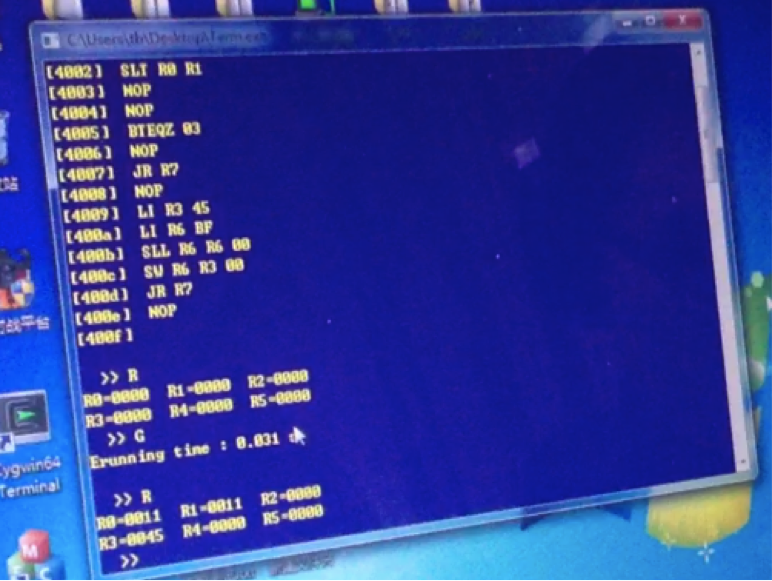
\includegraphics[width=1.1\columnwidth]{test.png}
\caption{扩展指令测试}
\label{fig:test}
\end{figure}

如图\ref{fig:test}所示,寄存器值发生了变化而且输出了字母E,因此程序成功运行

\subsection{VGA扩展运行结果}
\begin{figure}[h]
\centering
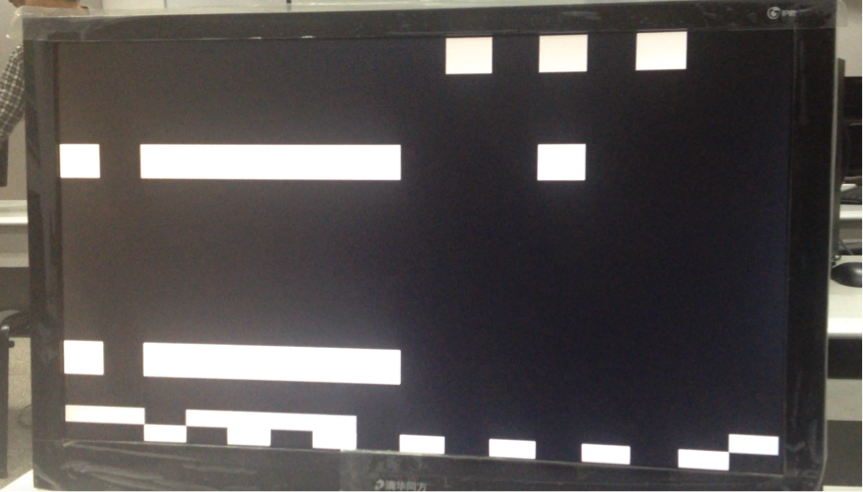
\includegraphics[width=1.1\columnwidth]{vga.png}
\caption{VGA扩展}
\label{fig:vga}
\end{figure}

我们用VGA模块在显示屏上显示寄存器信息
如图\ref{fig:vga}所示,从上到下依次为:PC、SP、IH、0-7号寄存器、当前运行指令的指令
通过按动按钮,我们可以观察到白块的移动,观察到寄存器值的变化,从而方便了程序的调试
详细运行情况请见result1.MOV

\section{实验总结}


%----------------------------------------------------------------------------------------
%	BIBLIOGRAPHY
%----------------------------------------------------------------------------------------

%\bibliographystyle{apalike}

%\bibliography{sample}

%----------------------------------------------------------------------------------------


\end{document}
